
%% Begin slides template file
\documentclass[11pt,t,usepdftitle=false,aspectratio=169]{beamer}
%% ------------------------------------------------------------------
%% - aspectratio=43: Set paper aspect ratio to 4:3.
%% - aspectratio=169: Set paper aspect ratio to 16:9.
%% ------------------------------------------------------------------

% \usepackage{enumitem}

\usetheme[nototalframenumber]{uibk}
%% ------------------------------------------------------------------
%% - foot: Add a footer line for conference name and date.
%% - logo: Add the university logo in the footer (only if 'foot' set).
%% - bigfoot/sasquatch: Larger font size in footer.
%% - nototalslidenumber: Hide the total number of slides (only if 'foot' set)
%% - license: Add CC-BY license symbol to title slide (e.g., for conference uploads)
%%   (TODO: At the moment no other licenses are supported.)
%% - licenseall: Add CC-BY license symbol to all subsequent slides slides
%% - url: use \url{} rather than \href{} on the title page
%% - nosectiontitlepage: switches off the behaviour of inserting the
%%   titlepage every time a \section is called. This makes it possible to
%%   use more than one section + thanks page and a ToC off by default.
%%   If the 'nosectiontitlepage' is set you can create UIBK title slides
%%   using the command '\uibktitlepage{}' in your document to create
%%   one or multiple title slides.
%% ------------------------------------------------------------------

%% ------------------------------------------------------------------
%% The official corporate colors of the university are predefined and
%% can be used for e.g., highlighting something. Simply use
%% \color{uibkorange} or \begin{color}{uibkorange} ... \end{color}
%% Defined colors are:
%% - uibkblue, uibkbluel, uibkorange, uibkorangel, uibkgray, uibkgraym, uibkgrayl
%% The frametitle color can be easily adjusted e.g., to black with
%% \setbeamercolor{titlelike}{fg=black}
%% ------------------------------------------------------------------

%\setbeamercolor{verbcolor}{fg=uibkorange}
%% ------------------------------------------------------------------
%% Setting a highlight color for verbatim output such as from
%% the commands \pkg, \email, \file, \dataset 
%% ------------------------------------------------------------------

\usepackage{tikz}
\usetikzlibrary{arrows,decorations.pathreplacing}
\tikzset{>=stealth}

% argument #1: any options
\newenvironment{customlegend}[1][]{%
    \begingroup
    % inits/clears the lists (which might be populated from previous
    % axes):
    \csname pgfplots@init@cleared@structures\endcsname
    \pgfplotsset{#1}%
}{%
    % draws the legend:
    \csname pgfplots@createlegend\endcsname
    \endgroup
}%

% makes \addlegendimage available (typically only available within an
% axis environment):
\def\addlegendimage{\csname pgfplots@addlegendimage\endcsname}

\tikzset{candidate/.style={draw, align=center, rounded corners=0.1cm, fill=white}}
\tikzset{balanced/.append style={draw=uibkorange, thick, fill=uibkorange!40}}
\tikzset{todo/.append style={draw=uibkorange, thick, pattern=north west lines, pattern color=uibkorang!40}}
\tikzset{target/.style={align=center, draw, thick, fill=white}}

\usepackage{adjustbox}
\usepackage{bm}
\usepackage{amsmath}
\usepackage{listings}
\lstset{escapechar=`}

\usepackage[norndcorners,customcolors]{hf-tikz}
\hfsetbordercolor{uibkorange}
\hfsetfillcolor{uibkorangel}

%% information for the title page ('short title' is the pdf-title that is shown in viewer's titlebar)
\title[Balancing binary values]{Defending against power analysis\\ by balancing binary values}
\subtitle{\large a compiler based approach}

\author[Alexander Schl\"ogl]{\small Alexander Schl\"ogl, supervised by Univ.-Prof. Dr. Rainer B\"ohme}
%('short author' is the pdf-metadata Author)
%% If multiple authors are required and the font size is too large you
%% can overrule the font size of author and url by calling:
%\setbeamerfont{author}{size*={10pt}{10pt},series=\mdseries}
%\setbeamerfont{url}{size*={10pt}{10pt},series=\mdseries}
%\URL{}
%\subtitle{}

\date{2019-09-11}

\headerimage{2}
%% ------------------------------------------------------------------
%% The theme offers four different header images based on the
%% corporate design of the university of innsbruck. Currently
%% 1, 2, 3 and 4 is allowed as input to \headerimage{...}. Default
%% or fallback is '1'.
%% ------------------------------------------------------------------

\usepackage{graphicx}
\graphicspath{ {fig/}}

\newcommand\blfootnote[1]{%
  \begingroup
  \renewcommand\thefootnote{}\footnote{#1}%
  \addtocounter{footnote}{-1}%
  \endgroup
}
\hyphenation{consumption}
\hyphenation{algorithm}

\newcommand{\hex}[1]{\texttt{0x#1}}

\renewcommand{\neg}[1]{\ensuremath{\overline{#1}}}
\newcommand{\bsep}{\; \| \; }
\newcommand{\borr}{\mathbin{\texttt{ORR}}}
\newcommand{\band}{\mathbin{\texttt{AND}}}
\newcommand{\bxor}{\mathbin{\texttt{XOR}}}
\newcommand{\bror}{\mathbin{\texttt{ROR}}}
\newcommand{\blsl}{\mathbin{\texttt{LSL}}}
\newcommand{\trans}[2]{\ensuremath{\texttt{transform\_#1\_#2}}}

\newcommand{\binp}[5]{\ensuremath{\%#1 &= #2 &&\bsep #3 &&\bsep #4 &&\bsep #5 &&}}
\newcommand{\btrans}[6]{\ensuremath{\%#1 &= #2 &&\bsep #3 &&\bsep #4 &&\bsep #5 && \;|\ #6}}

\newcommand{\vq}{\vphantom{q}}

\begin{document}

%% ALTERNATIVE TITLEPAGE
%% The next block is how you add a titlepage with the 'nosectiontitlepage' option, which switches off
%% the default behavior of creating a titlepage every time a \section{} is defined.
%% Then you can use \section{} as it's originally intended, including a table of contents.
% \usebackgroundtemplate{\includegraphics[width=\paperwidth,height=\paperheight]{titlebackground.pdf}}
% \begin{frame}[plain]
%     \titlepage
% \end{frame}
% \addtocounter{framenumber}{-1}
% \usebackgroundtemplate{}

%% Table of Contents, if wanted:
%% this requires the 'nosectiontitlepage' option and setting \section{}'s as you want them to appear here.
%% Subsections and subordinates are suppressed in the .sty at the moment, search
%% for \setbeamertemplate{subsection} and replace the empty {} with whatever you want.
%% Although it's probably too much for a presentation, maybe for a lecture.
%% Please note: \maketitle allows you to render a uibk-style title page wherever needed
%% in the document even if 'nosectiontitlepage' option is set (note: \maketitle will not
%% create a new section and is therefore not included in \tableofcontents (if used).
% \maketitle
% \begin{frame}
%     \vspace*{1cm plus 1fil}
%     \tableofcontents
%     \vspace*{0cm plus 1fil}
% \end{frame}


%% this sets the first PDF bookmark and triggers generation of the title page
\section{Motivation}
\begin{frame}
  \frametitle{Motivation}
  \begin{figure}
    \begin{columns}[T]
      \begin{column}{0.48\textwidth}
        \centering
        \vfill
        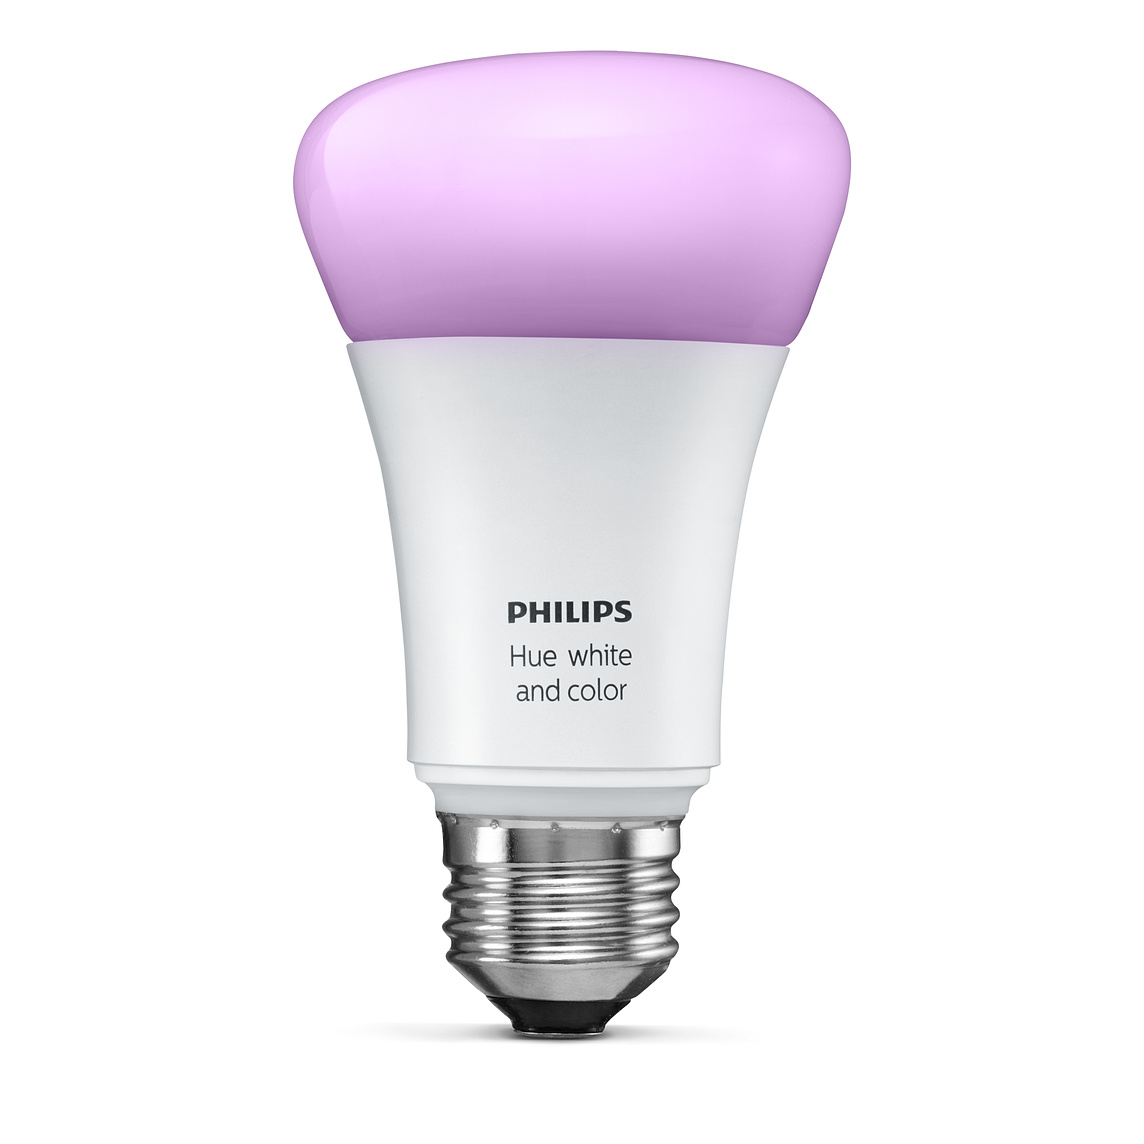
\includegraphics[width=0.8\textwidth]{hue.jpeg}
        \vfill
      \end{column}
      \hfill
      \begin{column}{0.48\textwidth}
        \centering
        \vspace{1cm}
        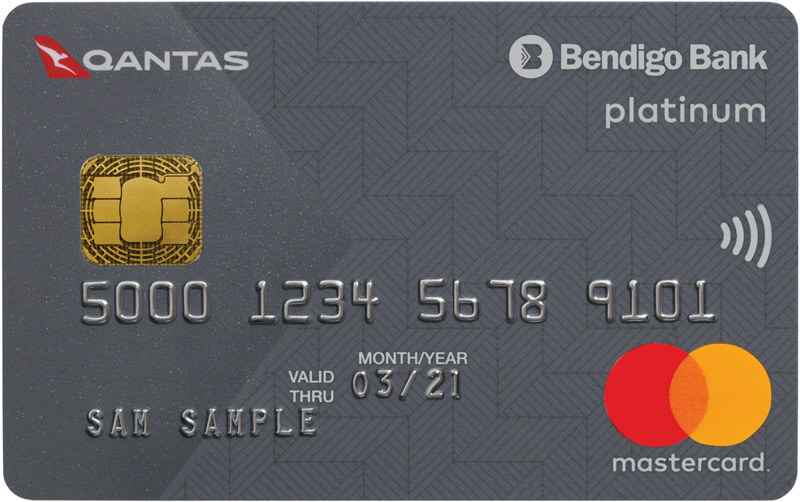
\includegraphics[width=0.7\textwidth]{bank-card.jpg}
        \vfill
      \end{column}
    \end{columns}
  \end{figure}
  \blfootnote{\tiny
https://store.storeimages.cdn-apple.com/4982/as-images.apple.com/is/HJCC2?wid=1144\&hei=1144\&fmt=jpeg\&qlt=95\&op\_usm=0.5,0.5\&.v=0}
  \blfootnote{\tiny
    https://www.liberaldictionary.com/wp-content/uploads/2019/01/bank-card-8123.jpg}
\end{frame}

\begin{frame}
  \frametitle{Motivation}
  \begin{figure}
    \centering
    \begin{tikzpicture}[every node/.style={draw}]
      \node (input) at (-3, 2) {\vq \only<1>{Input}\only<2>{\textcolor{uibkorange}{Known Input}}\only<3->{Known Input}};
      \node (secret) at (-3, -2) {\vq Secret};
      \node (result) at (-0.5,0) {\vq Result};
      \node[text width=2.5cm, align=center] (power) at (4,0) {\vq Power Consumption};

      \draw[->] (input) -- (result);
      \draw[->] (secret) -- (result);
      \draw[->] (result) -- (power);

      \onslide<2>{
        % \node[uibkorange,thick] (known) at (-1.5, 2) {\vq known};
        % \draw[->, uibkorange, line width=0.4mm] (known) -- (input);
        \draw[->, uibkorange, line width=0.4mm] (6,-3.5) -- (-4.5, -3.5) node[midway, above, draw=none] {Power Analysis Attack};
      }
      \onslide<3>{
        % \node[uibkblue, thick] (knownb) at (-1.5, 2) {\vq known};
        % \draw[->, uibkblue, line width=0.4mm] (knownb) -- (input);
        
        \draw[->, uibkblue, line width=0.4mm] (6,-3.5) -- (-4.5, -3.5) node[midway, above, draw=none] {Power Analysis Attack};
        \node[uibkorange, thick] (mask) at (-3, 0) {\vq Mask};
        \draw[uibkorange, thick, ->] (mask) -- (result);

        \draw[uibkorange, line width=0.4mm] (1.45,0.15) -- (1.15,-0.15);
        \draw[uibkorange, line width=0.4mm] (1.15,0.15) -- (1.45,-0.15);

        \draw[uibkorange, thick,<-] (1.3,-0.3) -- (1.3,-1) node[below, draw=none] {Dual-Rail Logic};
      }
    \end{tikzpicture}
  \end{figure}
\end{frame}

\begin{frame}
  \frametitle{Motivation}
  \vfill
  \begin{columns}[T]
    \begin{column}{0.48\textwidth}
      \begin{block}{Masking}
        Increases analysis complexity
        \begin{itemize}
        \item[+] Runs on standard hardware
        \item[--\hspace{0.4mm}] Built into algorithm
        \item[--\hspace{0.4mm}] Requires expert knowledge
        \end{itemize}
      \end{block}
    \end{column}
    %% \hfill
    \begin{column}{0.48\textwidth}
      \begin{block}{Dual-Rail Logic}
        Balances power consumption
        \begin{itemize}
        \item[+] Can run any program
        \item[--\hspace{0.4mm}] Requires specialized hardware
        \item[] \vq
        \end{itemize}
      \end{block}
    \end{column}
  \end{columns}
  \vfill
  \onslide<2>{
    \begin{alertblock}{Best of both worlds?}
      Apply balancing similar to Dual-Rail logic in software
    \end{alertblock}
  }
  \vfill
\end{frame}

%% this just generates PDF bookmarks
% \section{Overview}

%% first slide
\begin{frame}<1>[label=overview]
  \frametitle{Overview}
  \vfill
  \textbf{Content}

  \begin{itemize}
  \item Motivation
  \item \textcolor<2>{uibkorange}{Balancing}
  \item \textcolor<3>{uibkorange}{Arithmetic}
  \item \textcolor<4>{uibkorange}{Code Transformation}
  \item \textcolor<5>{uibkorange}{Results}
  \item \textcolor<6>{uibkorange}{Conclusion}
  \end{itemize}
  \vfill
\end{frame}

% \section{Balancing}
\begin{frame}
  \frametitle{Balancing}
  \vfill
  \textbf{Working assumption:}\\
  Power consumption is proportional to Hamming weight (number of 1s)\\
  $\rightarrow$ constant Hamming weight = constant power consumption
  \onslide<2->{
  \begin{alertblock}{Approach}
    Extend register size, and store inverse along with actual value
  \end{alertblock}
  \vspace{0.3cm}
  \begin{center}
    \begin{tikzpicture}
      \foreach \i in {0,8}{
        \draw (8-\i/4,0.2) -- (8-\i/4,-0.2);
        \node at (8-\i/4,-0.5) {\tiny \i};
      }
      \node at (7, 0) {\Large\texttt{x}};         

      \onslide<3>{
      \foreach \i in {16,24,32}{
        \draw (8-\i/4,0.2) -- (8-\i/4,-0.2);
        \node at (8-\i/4,-0.5) {\tiny \i};
      }
      \node at (5, 0) {\Large\texttt{0}};
      \node[uibkorange] at (3, 0) {\Large\neg{\texttt{x}}};
      \node at (1, 0) {\Large\texttt{0}};
      }
    \end{tikzpicture}
  \end{center}
  }
\end{frame}

% \againframe<3>{overview}

% \section{Arithmetic}
\begin{frame}
  \frametitle{Arithmetic}
  Regular operators will not work:
  \begin{center}
    \begin{tikzpicture}
      \foreach \y in {2,0,-2}{
        \foreach \i in {0,8,...,32}{
          \draw (8-\i/4,\y+0.2) -- (8-\i/4,\y-0.2);
          \node at (8-\i/4,\y-0.5) {\tiny \i};
        }
        \node at (5, \y) {\Large\texttt{0}};
        \node at (1, \y) {\Large\texttt{0}};
      }
      \node at (7, 2) {\Large\texttt{x}};
      \node at (3, 2) {\Large\neg{\texttt{x}}};

      \node at (4,.8) {\Large{$\bm{\lor}$}};

      \node at (7, 0) {\Large\texttt{y}};
      \node at (3, 0) {\Large\neg{\texttt{y}}};

      \node at (4,-1.2) {\Large{$\bm{=}$}};

      \node at (7, -2) {\Large$\texttt{x} \bm{\lor} \texttt{y}$};
      \node at (3, -2) {\Large$\neg{\texttt{x}} \bm{\lor} \neg{\texttt{y}}$};

      \node[uibkorange] at (3, -2.6) {\Large$\bm{\neq}$};
      \node at (3.91, -3.2) {\Large$\neg{\texttt{x} \bm{\lor} \texttt{y}} = \neg{\texttt{x}} \bm{\land} \neg{\texttt{y}}$};
  \end{tikzpicture}
  \end{center}
\end{frame}

\begin{frame}[fragile]
  \frametitle{Arithmetic}

  \begin{columns}[T] % align columns
    \begin{column}{.28\textwidth}
      Find replacements for:
      \begin{itemize}
      \item \textcolor<2>{uibkorange}{\texttt{ORR}} \only<2>{\quad\tikz[baseline=0.5ex]{\draw[->,uibkorange,line width=0.3mm] (0,0.2) -- (2,0.2);}}
      \item \texttt{AND}
      \item \texttt{XOR}
      \item \texttt{ADD}
      \item \texttt{SUB}
      \item \texttt{MUL}
      \item \texttt{SHIFTS}
      \item \texttt{DIV}
      \item \texttt{REM}
      \end{itemize}
    \end{column}%
    \hfill%
    \pause
    \vrule
    \hfill
    \begin{column}{.6\textwidth}
      \vspace{1cm}
      \begin{lstlisting}[language=C, basicstyle=\small]
int balanced_or(int lhs,
        int rhs) {
  int temp_or = lhs | rhs;
  int temp_and = lhs & rhs;
  int combined = (temp_and << 8)
          | temp_or;
  combined &= 0xff0000ff;
  return balanced_2_1(combined);
}
      \end{lstlisting}
    \end{column}
  \end{columns}
\end{frame}

\begin{frame}
  \frametitle{Verifying the arithmetic}
  Perform exhaustive search of the input space:
  \begin{columns}[T]
    \begin{column}{0.48\textwidth}
      \begin{block}{Test framework}
        \begin{itemize}
        \item Takes individual steps as lambdas
        \item Executes over all inputs
        \item Stores intermediate values
        \item \textcolor<2>{uibkorange}{Checks correctness}
        \item \textcolor<3>{uibkorange}{Plots Hamming weight histograms}
        \end{itemize}        
      \end{block}
    \end{column}
    \hfill
    \onslide<3>{
    \begin{column}{0.48\textwidth}
      \centering
      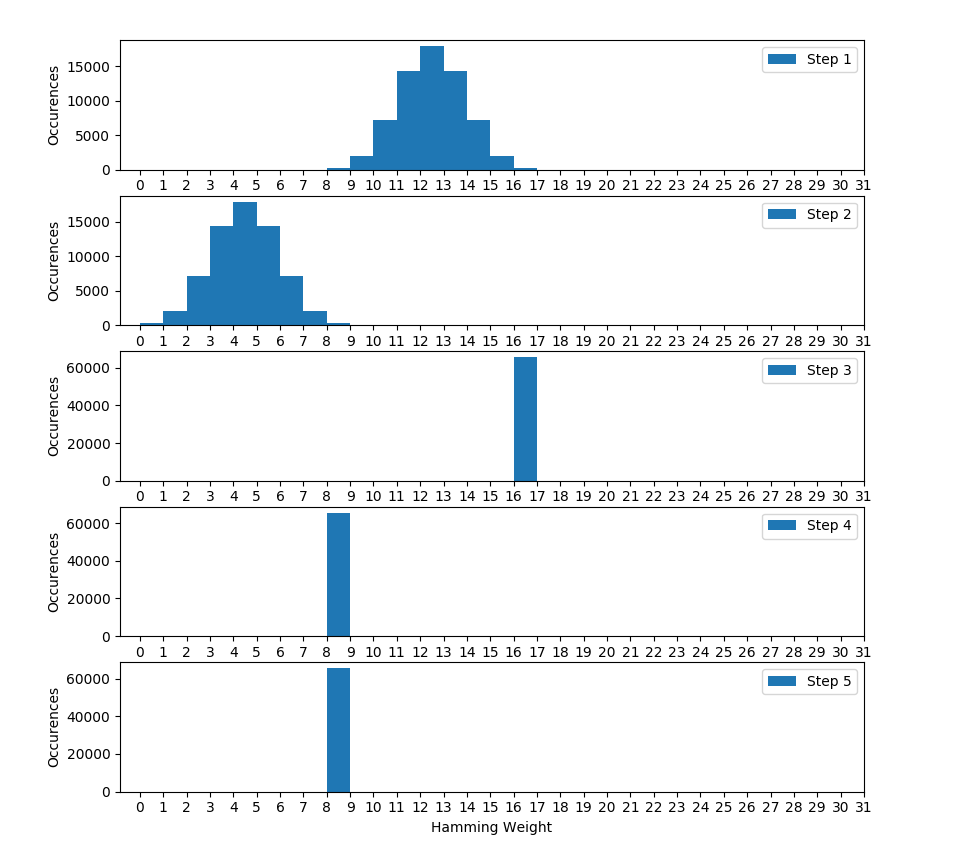
\includegraphics[width=\textwidth]{orr.png}
    \end{column}
    }
  \end{columns}
\end{frame}

% \againframe<4>{overview}

% \section{Code Transformation}
\begin{frame}
  \frametitle{Applying the changes}
  \begin{alertblock}{Automatic balancing}
    Rewrite code during compilation
  \end{alertblock}

  \vfill
  \onslide<2->{
  LLVM:
  \begin{figure}
  \centering
  \begin{tikzpicture}
    \node[draw, minimum width=1.3cm, minimum height=0.6cm] at (-2.5,1.5) (C) {C};
    \node[draw, minimum width=1.3cm, minimum height=0.6cm] at (-2.5,0.5) (C++) {C++};
    \node[draw, minimum width=1.3cm, minimum height=0.6cm] at (-2.5, -0.5) (Haskell) {Haskell};
    \node[draw, minimum width=1.3cm, minimum height=0.6cm] at (-2.5, -1.5) (otherl) {...};
    \node[draw] at (-0.75, 0) (irl) {IR};

    \draw[decoration={brace,mirror,amplitude=6pt}, decorate, line width=0.3mm, uibkgray!70] (-3.3,-1.9) -- (-1.7, -1.9) node[midway, below, yshift=-3pt] {\scriptsize Frontends};
    
    \node[draw, label=Optimizer Passes, minimum width=4cm, minimum height=1.3cm] at (2,0) (optimization) {};
    \node[draw, minimum size=0.5cm] at (0.6,0) {};
    \node[draw, minimum size=0.5cm] at (1.2,0) {};
    \node[draw, minimum size=0.5cm] at (1.8,0) {};
    \node[draw, minimum size=0.5cm] at (2.4,0) {};
    \node at (3.0, 0) {...};

    \node[draw] at (4.75, 0) (irr) {IR};
    \node[draw, minimum width=1.3cm, minimum height=0.6cm] at (6.5,1) (x86) {x86};
    \node[draw, minimum width=1.3cm, minimum height=0.6cm] at (6.5,0) (arm) {ARM};
    \node[draw, minimum width=1.3cm, minimum height=0.6cm] at (6.5,-1) (otherr) {...};

    \draw[decoration={brace,mirror,amplitude=6pt}, decorate, line width=0.3mm, uibkgray!70] (5.7,-1.9) -- (7.3, -1.9) node[midway, below, yshift=-3pt] {\scriptsize Backends};
    
    \draw[->] (C) -- (irl);
    \draw[->] (C++) -- (irl);
    \draw[->] (Haskell) -- (irl);
    \draw[->] (otherl) -- (irl);

    \draw[->] (irl) -- (optimization);
    \draw[->] (optimization) -- (irr);

    \draw[->] (irr) -- (x86);
    \draw[->] (irr) -- (arm);
    \draw[->] (irr) -- (otherr);

    \onslide<3>{
    \node[draw, minimum height=0.6cm] (balance) at (3,-2) {Balance.cpp};
    \draw[->, uibkorange, line width=0.3mm, shorten <= 5pt] (balance) -- (3,-0.2);
    }
  \end{tikzpicture}
  \end{figure}
  }
\end{frame}

\begin{frame}
  \frametitle{Optimizer Pass}
  \centering
  \begin{tikzpicture}[scale=0.6, every node/.style={transform shape}]
    \draw[fill=uibkblue!10] (1.7, 0.4) ellipse (7cm and 5.7cm);
    \node[align=center] at (-2.8, -2.1) {HEAP / GLOBALS};

    \draw[fill=uibkorange!10] (1.2,2) ellipse (5.7cm and 3.7cm);
    \node at (-1.7, 0) {STACK / LOCALS};

    \node at (-4.5, -4.2) {BUSSES};

    \node (literals) [candidate] at (-1.7,3.7) {literals};
    \node (ops) [candidate] at (-3,1.5) {binary \\ operations};
    \node (lvars) [candidate] at (0.8,2) {local \\ variables};
    \node (larrs) [candidate] at (1.7,-0.5) {local \\ arrays};
    \node (params) [candidate] at (3.5, 4) {function \\ parameters};
    \node (returns) [candidate] at (4, 2.5) {return \\ values};
    \node (registers) [target] at (4.3, 0) {registers};

    \draw[->] (literals) -> (lvars);
    \draw[->] (ops) -> (lvars);
    \draw[->] (lvars) -> (larrs);
    \draw[<->] (lvars) -> (params);
    \draw[<->] (lvars) -> (returns);

    \draw[->] (lvars) -> (registers);
    \draw[->] (larrs) -> (registers);

    \node (gvars) [candidate] at (0.5, -2.7) {global \\variables};
    \node (garrs) [candidate] at (3.2, -2.6) {global \\arrays};
    \node (constants) [candidate] at (0.8, -3.9) {constants};
    \node (memory) [target] at (3.4, -4.2) {main \\memory};
    \node (pointers) [candidate] at (6.9, -1.0) {pointers};

    \draw[->] (lvars) -> (gvars);
    \draw[->] (larrs) -> (garrs);
    \draw[->] (constants) -> (gvars);
    \draw[->] (gvars) -> (memory);
    \draw[->] (garrs) -> (memory);

    \node (databus) [target] at (6.7, -4.7) {data \\ bus};
    \node (addressbus) [target] at (8.9, -3.0) {address \\ bus};

    \draw[->] (registers) -> (databus);
    \draw[->] (memory) -> (databus);
    \draw[->] (pointers) -> (addressbus);
  \end{tikzpicture}
\end{frame}

\begin{frame}[label=implemented]
  \frametitle{Optimizer Pass}
  \centering
  \begin{tikzpicture}[scale=0.6, every node/.style={transform shape}]
    \draw[fill=uibkblue!10] (1.7, 0.4) ellipse (7cm and 5.7cm);
    \node[align=center] at (-2.8, -2.1) {HEAP / GLOBALS};

    \draw[fill=uibkorange!10] (1.2,2) ellipse (5.7cm and 3.7cm);
    \node at (-1.7, 0) {STACK / LOCALS};

    \node at (-4.5, -4.2) {BUSSES};

    \node (literals) [candidate, balanced] at (-1.7,3.7) {literals};
    \node (ops) [candidate, balanced] at (-3,1.5) {binary \\ operations};
    \node (lvars) [candidate, balanced] at (0.8,2) {local \\ variables};
    \node (larrs) [candidate, balanced] at (1.7,-0.5) {local \\ arrays};
    \node (params) [candidate, balanced] at (3.5, 4) {function \\ parameters};
    \node (returns) [candidate, balanced] at (4, 2.5) {return \\ values};
    \node (registers) [target, balanced] at (4.3, 0) {registers};

    \draw[->] (literals) -> (lvars);
    \draw[->] (ops) -> (lvars);
    \draw[->] (lvars) -> (larrs);
    \draw[<->] (lvars) -> (params);
    \draw[<->] (lvars) -> (returns);

    \draw[->] (lvars) -> (registers);
    \draw[->] (larrs) -> (registers);

    \node (gvars) [candidate] at (0.5, -2.7) {global \\variables};
    \node (garrs) [candidate] at (3.2, -2.6) {global \\arrays};
    \node (constants) [candidate] at (0.8, -3.9) {constants};
    \node (memory) [target] at (3.4, -4.2) {main \\memory};
    \node (pointers) [candidate] at (6.9, -1.0) {pointers};

    \draw[->] (lvars) -> (gvars);
    \draw[->] (larrs) -> (garrs);
    \draw[->] (constants) -> (gvars);
    \draw[->] (gvars) -> (memory);
    \draw[->] (garrs) -> (memory);

    \node (databus) [target] at (6.7, -4.7) {data \\ bus};
    \node (addressbus) [target] at (8.9, -3.0) {address \\ bus};

    \draw[->] (registers) -> (databus);
    \draw[->] (memory) -> (databus);
    \draw[->] (pointers) -> (addressbus);
  \end{tikzpicture}
\end{frame}

\begin{frame}
  \frametitle{Optimizer Pass}

  \vfill
  Additionally transform:
  \begin{itemize}
  \item stores
  \item loads
  \item casts
  \item array indexing
  \item compares
  \item function calls
  \end{itemize}
  \vfill
\end{frame}

% \section{Results}
\begin{frame}
  \frametitle{Evaluation}

  How to generate ``virtual'' power traces?
  
  \begin{block}{Qemu alone}
    \begin{itemize}
    \item[+] fast
    \item[--\hspace{0.4mm}] incorrect view
    \end{itemize}
  \end{block}
  \pause
  \begin{alertblock}{Qemu + gdb}
    \begin{itemize}
    \item[+] correct view
    \item[+] includes program location information
    \item[--\hspace{0.4mm}] \textbf{very} slow
    \end{itemize}
    Execute instruction by instruction, dump registers every time
  \end{alertblock}
\end{frame}

\begin{frame}[label=results]
  \frametitle{Results}
  \begin{alertblock}{No attack}
    No attack was mounted, instead performed statistical analysis
  \end{alertblock}
  \center
  \onslide<2->{
  \vfill
  \begin{tabular}{|l|l|l|}
    \hline
    & \multicolumn{2}{c|}{AES} \\
    \cline{2-3}
    & unbalanced & balanced \\
    \cline{2-3}
    Executed instructions & 22 876 & 339 168 \\
    Relative increase & 1 & 14.888 \\
    Balanced operations & 20 571 & 334 521 \\
    Balancedness      & 0.903 & 0.986 \\
    Unbalanced operations & 2211 & 4647 \\
    \hline
  \end{tabular}
  }
  \vfill
\end{frame}

% \againframe<4>{results}

% \section{Conclusion}
% \againframe<6>{overview}

\begin{frame}
  \frametitle{Summary}
  \vfill
  \begin{itemize}
  \item Arithmetic is \emph{mostly} proven to be correct
  \item Works without programmer work
  \item Balances everything on stack
  \item Requires more powerful, but standard hardware
  \item Does not explode code size
  \end{itemize}
  \vfill
\end{frame}

\begin{frame}
  \frametitle{Limitations}
  \vfill
  \begin{itemize}
  \item Works only on stack
  \item Only tested on some code samples
  \item Correctness of \texttt{REM} and \texttt{DIV} not proven
  \item Not attacked, only evaluated
  \item Greatly increased execution time
  \end{itemize}
  \vfill
\end{frame}

\begin{frame}
  \frametitle{Future work}
  Improve on thesis:
  \begin{itemize}
  \item Test on actual hardware
  \item Balance globals
  \item Improve operators
  \item Mark balancing targets
  \end{itemize}
  \vspace{0.5cm}
  Similar ideas:
  \begin{itemize}
  \item Move balancing to type system
  \item Other power analysis defenses
  \item Control flow randomization
  \item Move more security tools to LLVM
  \end{itemize}
\end{frame}

\begin{frame}
  \frametitle{Conclusion}
  \begin{itemize}
  \item Debugging optimizer passes is hard
  \item Security and performance likely mutually exclusive
  \item Backend cannot entirely be ignored
  \item Qemu is not a processor emulator
  \end{itemize}
  \vfill
  \begin{block}{LLVM IR}
    LLVM's intermediate representation offers many avenues for future work,\\
    not only for optimizition, but also for security.
  \end{block}
\end{frame}

\begin{frame}
\end{frame}

\appendix

\begin{frame}
  \begin{figure}
    \centering
    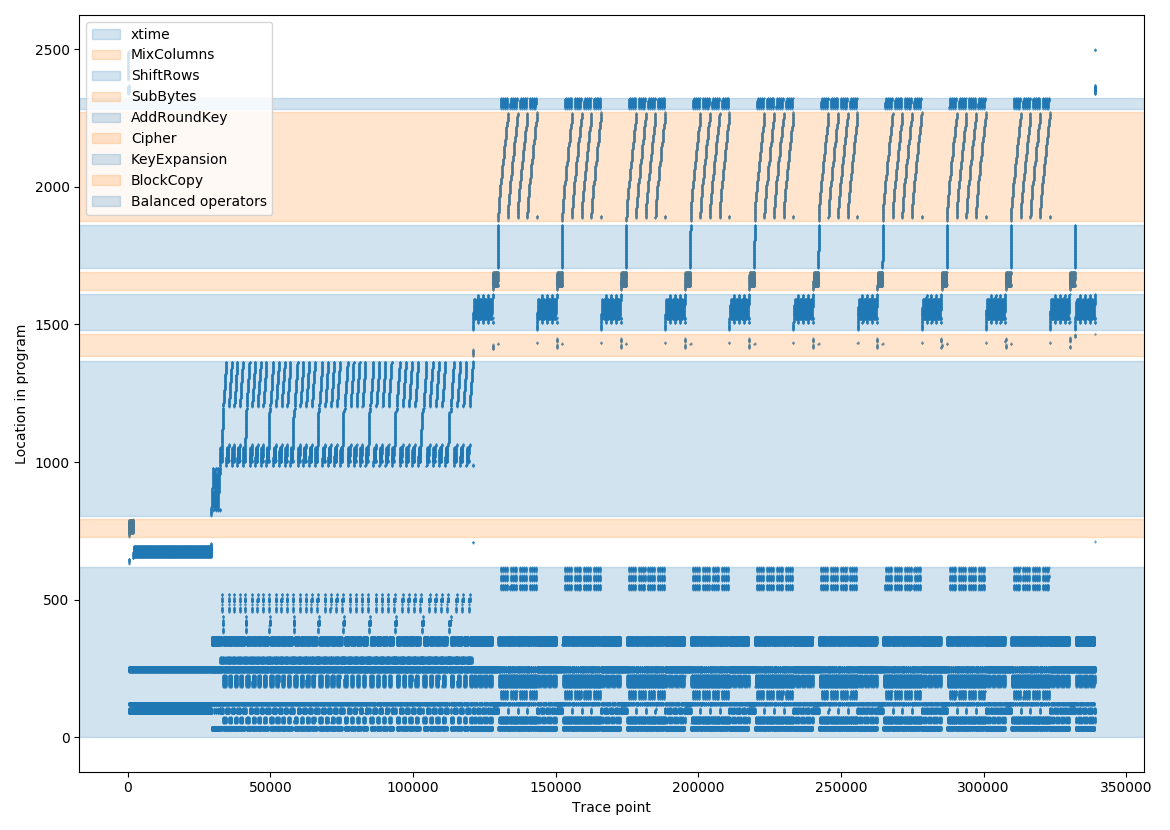
\includegraphics[height=\textheight]{aes-parts.png}
  \end{figure}
\end{frame}

\begin{frame}
  \begin{figure}
    \centering
    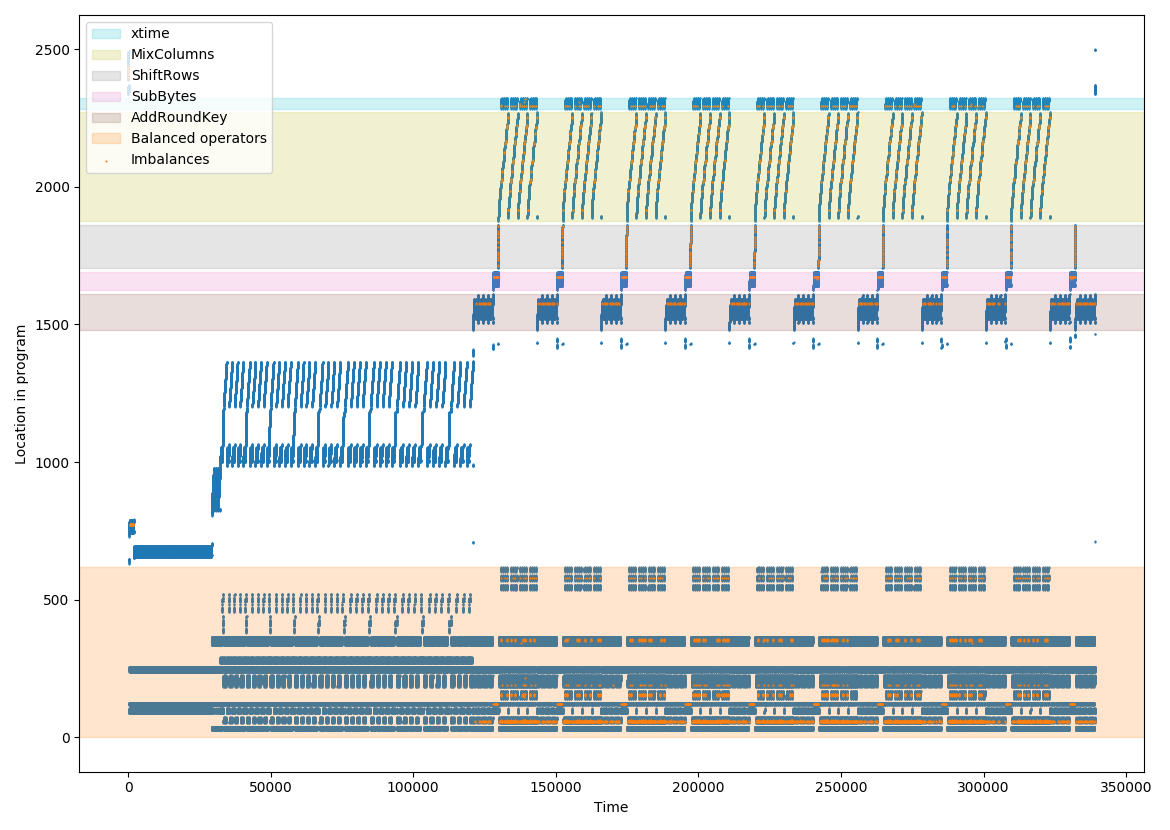
\includegraphics[height=\textheight]{imbalances-0.png}
  \end{figure}
\end{frame}

\begin{frame}
  \begin{figure}
    \centering
    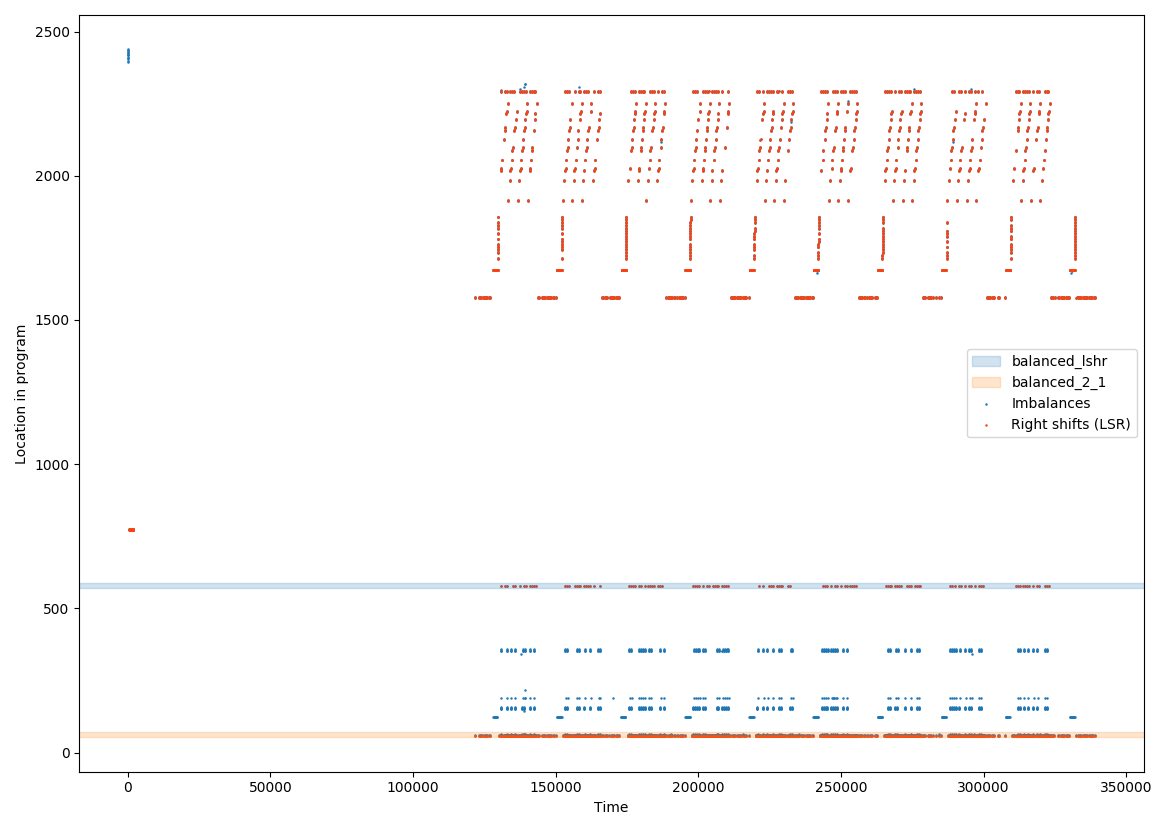
\includegraphics[height=\textheight]{imbalances-1.png}
  \end{figure}

\end{frame}
\begin{frame}
  \begin{figure}
    \centering
    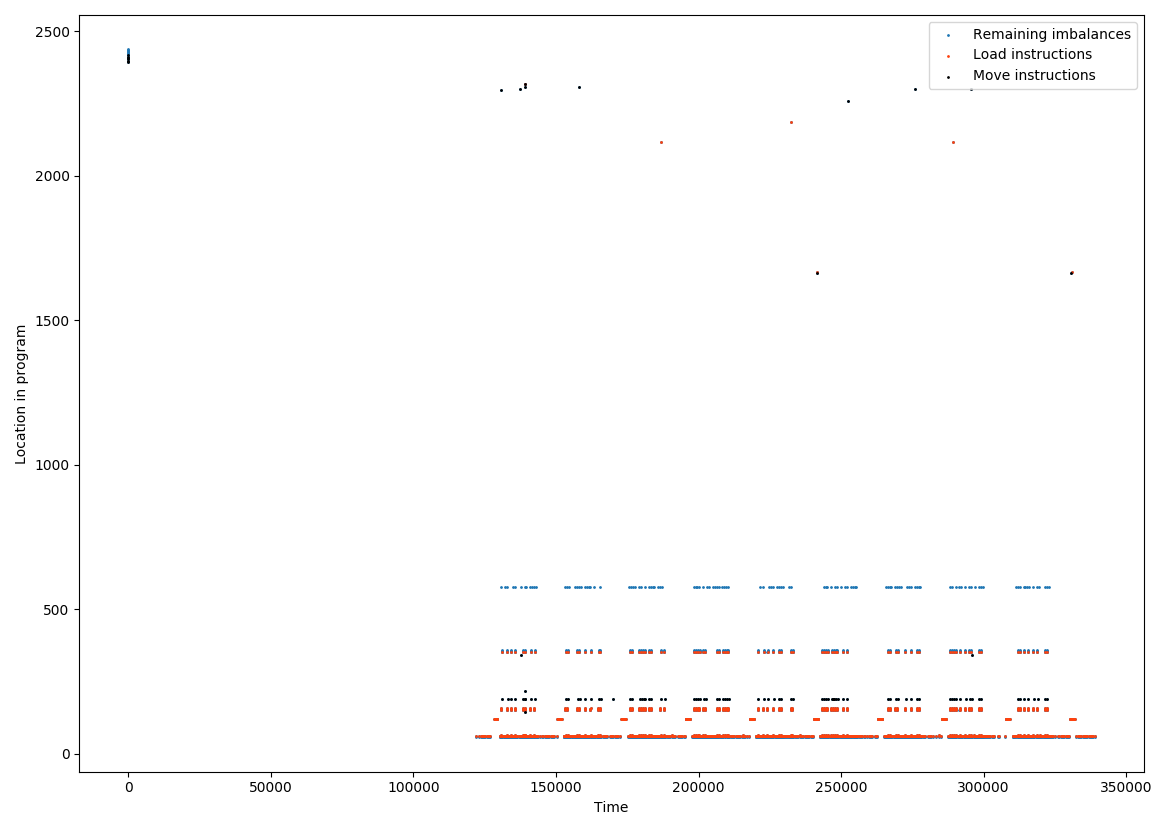
\includegraphics[height=\textheight]{imbalances-2.png}
  \end{figure}

\end{frame}
\begin{frame}
  \begin{figure}
    \centering
    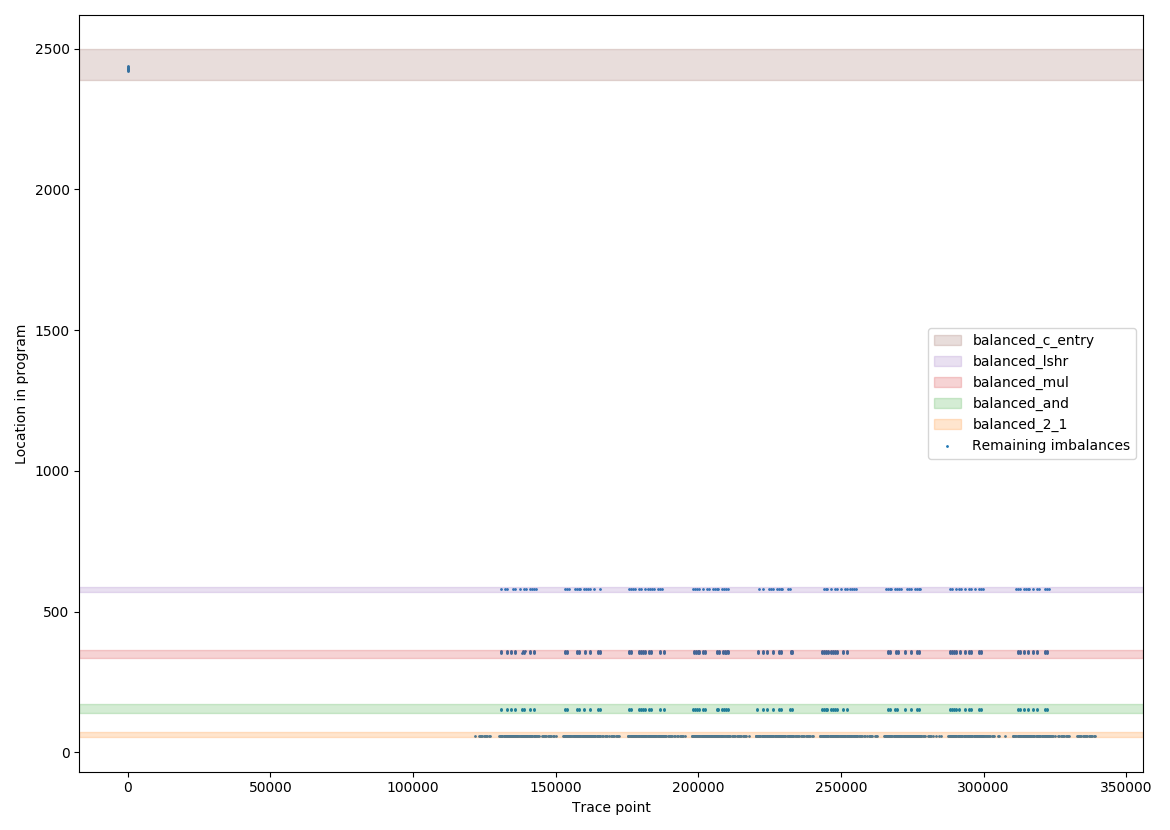
\includegraphics[height=\textheight]{imbalances-3.png}
  \end{figure}
\end{frame}

\begin{frame}[label=results]
  \frametitle{Results}
  \begin{alertblock}{No attack}
    No attack was mounted, instead performed statistical analysis
  \end{alertblock}
  \center
  \vfill
  \begin{tabular}{|l|c|c|c|}
    \hline
    & \multicolumn{3}{c|}{AES} \\
    \cline{2-4}
    & unbalanced & balanced & filtered balanced \\
    \cline{2-4}
    Executed instructions & 22 876 & 339 168 & 339 168\\
    Relative increase & 1 & 14.888 & 14.888 \\
    Balanced operations & 20 571 & 334 521 & 337 852\\
    Unbalanced operations & 2211 & 4647 & 1316 \\
    Balancedness      & 0.903 & 0.986 & 0.996\\
    \hline
  \end{tabular}
  \vfill
\end{frame}

\section{Power Analysis}
\label{poweranalysis}

In most cases the power consumption during execution is data-dependent.
Setting a bit to 1 requires more power than setting it to 0.
Power consumption is thus directly linked to the \hammingw{} of processed data.
An attacker can then measure the power consumption and make inferences on the data being processed.

Performing \poweranalysis{} requires some setup:
An attacker solders a resistor between the target processor and the ground of its power supply.
She then measures the voltage difference between both ends with an oscilloscope (this voltage is directly proportional to the current flowing through the resistor).
This gives her easy access to the power traces at a high resolution and for every clock cycle.

With these power traces an attacker then has the choice of multiple attack forms of varying complexity.\cite{kocher1998introduction}\cite{brier2004correlation}
The simplest form is \emph{Simple \poweranalysis{}} (SPA), and it involves directly examining the power consumption.
As large control blocks can be identified, a data-dependent control flow can leak information this way.
An example target would be RSA decryption being calculated via the square-and-multiply algorithm.
The difference between the multiply and the square operation is directly observable from a single power trace.
As the order of these operations is linked to the private key, identifying the control flow leaks the private key.
\Cref{fig:spa} shows a trace for square-and-multiply in RSA decryption, including the leaked private key bits.

\begin{figure}[h]
  \centering
  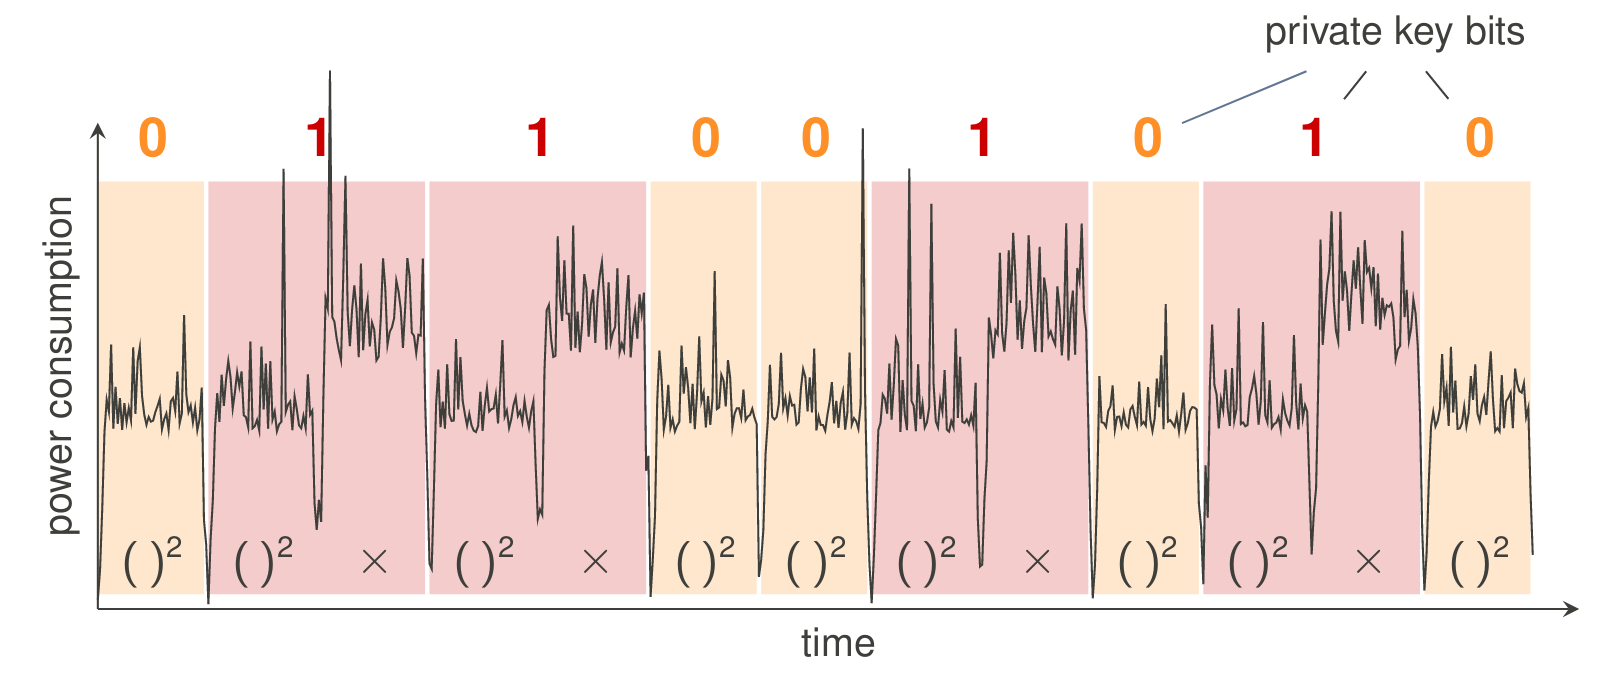
\includegraphics[width=\textwidth]{spa.png}
  \caption{Simple Power Analysis on square-and-multiply RSA\cite{boehme2017netsec}}
  \label{fig:spa}
\end{figure}

The control flow is often not enough to leak the entire secret, and it is very hard to gain information about the actual data from only SPA.
For this a more complex variant of \poweranalysis{} can be used, namely \emph{Differential \poweranalysis{}} (DPA).
DPA requires a large number of traces, with one factor for the power consumption known.
For cryptographic operations this equates a \emph{chosen plaintext} attack scenario.

DPA then attacks the individual bits of the key.
The attacker considers two cases, one for each value of the current key bit.
First she assumes the value of the current key bit is 0.
She then chooses a bitwise operation (e.g. XOR of the plaintext with the key in the first round of AES), and splits the power traces into two sets, based on the value of the target bit in the expected result of this operation.
Next she calculates the mean power consumption of both sets.
As the value of the other bits, as well as other factors for the power consumption, are randomly distributed, calculating the mean will neutralize them.
If her assumption was correct, the difference of both means will exhibit a spike at the time of the chosen operation.
Either way, the value of the current key bit is revealed to her.

\Cref{fig:dpa} shows a typical DPA result with the mean power consumptions of both sets, the difference between the two, and the difference with the Y axis magnified by a factor of 15.
This analysis was performed on the output of the least significant bit after the first S-box substitution in AES.

\begin{figure}[h]
  \centering
  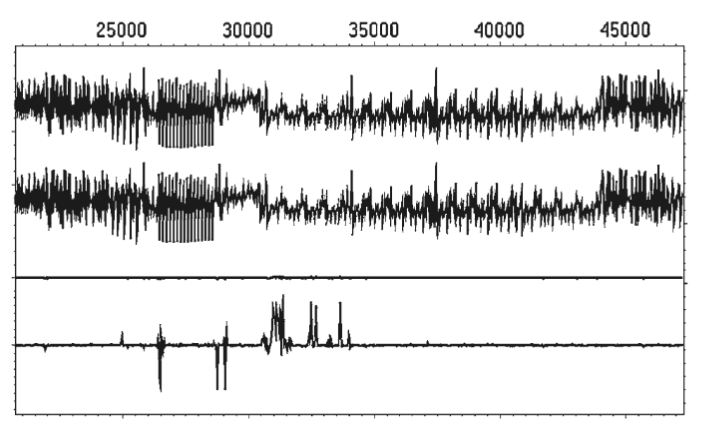
\includegraphics[width=0.8\textwidth]{dpa.png}
  \caption{Difference in means during DPA\cite{kocher2011introduction}}
  \label{fig:dpa}
\end{figure}

Even more higher order information about the key can be found with \emph{Correlational \poweranalysis{}} (CPA).
CPA is the most complex of these attacks, but also offers the best results.
The attacker starts by making a list of candidate values for every byte of the key.
Attacking individual bytes at a time, instead of the whole key, still keeps the required effort feasible.
As she knows which algorithm she is attacking, she knows which operations will take place, and can calculate expected intermediate results based on her chosen plaintexts and key candidates.
She can then calculate the expected power consumptions for these intermediate results.

The attacker can now calculate the correlation between the expected power consumptions for every key byte candidate and the actual power consumption.
The candidate with the highest correlation coefficient is then the most probable value for the current key byte.

\subsection{Defenses against \poweranalysis{} attacks}
\poweranalysis{} works because processed data directly influences the power consumption.
Defenses against this class of attack usually work by either adding additional factors to the power consumption, thus increasing the computational effort required for analysis, or by reducing variances in power consumption altogether.
This reduced variance decreases the information an attacker can gain from the same number of power traces, giving her reduced confidence in her result or requiring her to capture more traces.

Masking\cite{golic2002multiplicative}\cite{coron2000boolean} for example is an algorithm specific defensive measure that adds a third factor to the power consumption by first performing adding a masking value to the plaintext via an invertible operation.
The cryptographic algorithm then works on the masked value, and only in the end unmasks the result.
As such the attacker has to calculate her correlation for each possible combination of key byte and mask value.
This increases the number of traces she needs to capture (to still provide the same confidence in her analysis) and the computation time of her analysis.

Other defensive measures focus on creating a worse signal to noise ratio for the entire power consumption.
One technique that has gained a lot of traction is \dual{}\cite{sokolov2005design}.
It works by calculating the inverse of every intermediate result along with the actual result, thus balancing the number of 1s.
This results in a constant \hammingw{} and therefore a data-independent power consumption.

Unfortunately, \dual{} suffers from multiple engineering problems.
The power required to set the value of a bit to 1 is dependent on properties of the underlying transistors, which are subject to variances in manufacturing.\cite{razafindraibe2006formal}
Minimal differences in clock timings between both paths can also reduce the security of \dual{}\cite{baddam2008path}.
Storing the inverse also requires significantly larger circuitry, doubling the circuit size or more\cite{baddam2008path}.

Even with these caveats, \dual{} has the major advantage that once it is applied, \emph{any} code can be run without modifications while still benefiting from the increased robustness.

\end{document}
